\section{State Estimation for Robotics} \label{stateEstimator}

\hspace{2cm}A typical control system requires actual state measurement to perform the required task correctly. A robot pose represents its state for example. Due to sensor capabilities, measurement noise, and model uncertainty, it is not possible to know an actual state exactly. So, it is required to estimate system state from all uncertain  information about it. A state estimator is typically a computer implemented mathematical model and it provides the estimation of the internal states of the system. In most practical cases, the physical state of the system cannot be determined by direct observation. Instead, indirect effects of the internal state are observed by way of the system outputs.\cite{stateEstimator}
\par
We are using robot localization as state estimation, localization is the process of determining the position of the mobile robot by using sensor fusion concept. Sensor fusion is software that intelligently combines data from several sensors.\cite{web034}
\par
Using more sensors, increase the accuracy of localization algorithm (accurately locate the mobile robot) as shown in the figure below:


 \begin{figure}[H]%
    \center%
    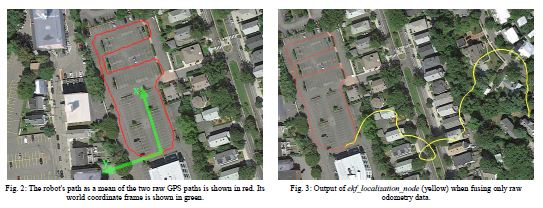
\includegraphics[width=.9\textwidth]{images/Alaa/sensorFusion0.JPG}%
  \end{figure}
  
 \begin{figure}[H]%
    \center%
    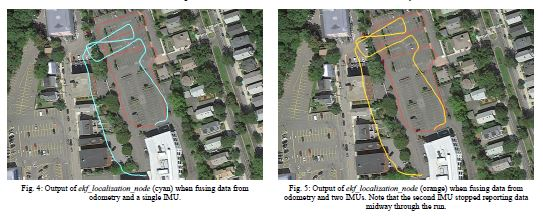
\includegraphics[width=.9\textwidth]{images/Alaa/sensorFusion1.JPG}%
  \end{figure}
  
   \begin{figure}[H]%
    \center%
    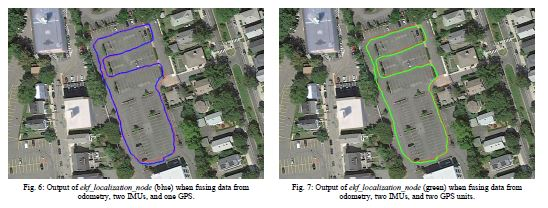
\includegraphics[width=.9\textwidth]{images/Alaa/sensorFusion2.JPG}%
     % you need to add the caption for the list of figures
    \caption[Sensor Fusion]{increasing number of sensors leads to increase the accuracy of locating the robot.}\cite{web035}\label{fig: Sensor Fusion}%
  \end{figure}
  
A stable and robust outdoor localization algorithm is critical to successful outdoor navigation. However, unpredictable external effects and interruption of the GPS signal cause difficulties in outdoor localization. So this is the reason of using multiple sensors on localization as we discussed previously in the so-called Sensor Fusion.
In our project we used the localization package integrated with ROS (robot\_pose\_ekf package).

\subsection {Extended Kalman Filter (EKF)}
\hspace{2cm} Most of the modern systems are equipped with numerous sensors that provide estimation of hidden (unknown) variables based on the series of measurements. For example, the GPS receiver provides the location and velocity estimation, where location and velocity are the hidden variables and differential time of satellite's signals arrival are the measurements.

One of the biggest challenges of tracking and control system is to provide accurate and precise estimation of the hidden variables in presence of uncertainty. In the GPS receiver, the measurements uncertainty depends on many external factors such as thermal noise, atmospheric effects, slight changes in satellite's positions, receiver clock precision and many more.

Kalman Filter is one of the most important and common estimation algorithms. The Kalman Filter produces estimates of hidden variables based on inaccurate and uncertain measurements. As well, the Kalman Filter provides a prediction of the future system state, based on the past estimations.

The filter is named after Rudolf E. Kalman (May 19, 1930 – July 2, 2016). In 1960, Kalman published his famous paper describing a recursive solution to the discrete-data linear filtering problem. \cite{kalmanFilter}\\

In our project we used extended Kalman filter (EKF) which is the nonlinear version of the Kalman filter that linearizes about an estimate of the current mean and covariance. In the extended Kalman filter, the state transition and observation models don't need to be linear functions of the state but may instead be differentiable functions:\\
     ${\displaystyle {\boldsymbol {x}}_{k}=f({\boldsymbol {x}}_{k-1},{\boldsymbol {u}}_{k})+{\boldsymbol {w}}_{k}} \\
   {\displaystyle {\boldsymbol {z}}_{k}=h({\boldsymbol {x}}_{k})+{\boldsymbol {v}}_{k}} \\ $
Here $w_k$ and $v_k$ are the process and observation noises which are both assumed to be zero mean multivariate Gaussian noises with covariance $Q_k$ and $R_k$ respectively. $u_k$ is the control vector.
The function $f$ can be used to compute the predicted state from the previous estimate and similarly the function $h$ can be used to compute the predicted measurement from the predicted state. However, $f$ and $h$ cannot be applied to the covariance directly. Instead a matrix of partial derivatives (the Jacobian) is computed.\\
At each time step, the Jacobian is evaluated with current predicted states. These matrices can be used in the Kalman filter equations. This process essentially linearizes the non-linear function around the current estimate.\cite{extendedKalmanFilter}\\
\textbf{Discrete-time predict and update equations:}\\
Notation  ${\displaystyle {\hat {\mathbf {x} }}_{n\mid m}} $represents the estimate of ${\displaystyle \mathbf {x} }$ at time $n$ given observations up to and including at time $m \leq n$. \\
\textbf{Predict}\\
Predicted state estimate:  	 ${\displaystyle {\hat {\boldsymbol {x}}}_{k|k-1}=f({\hat {\boldsymbol {x}}}_{k-1|k-1},{\boldsymbol {u}}_{k})}$ \\
Predicted covariance estimate: ${\displaystyle {\boldsymbol {P}}_{k|k-1}={{\boldsymbol {F}}_{k}}{\boldsymbol {P}}_{k-1|k-1}{{\boldsymbol {F}}_{k}^{\top }}+{\boldsymbol {Q}}_{k}}$ \\
\textbf{Update}\\
Innovation or measurement residual: ${\displaystyle {\tilde {\boldsymbol {y}}}_{k}={\boldsymbol {z}}_{k}-h({\hat {\boldsymbol {x}}}_{k|k-1})}$ \\
Innovation (or residual) covariance: ${\displaystyle {\boldsymbol {S}}_{k}={{\boldsymbol {H}}_{k}}{\boldsymbol {P}}_{k|k-1}{{\boldsymbol {H}}_{k}^{\top }}+{\boldsymbol {R}}_{k}} $ \\
Near-optimal Kalman gain: $ {\displaystyle {\boldsymbol {K}}_{k}={\boldsymbol {P}}_{k|k-1}{{\boldsymbol {H}}_{k}^{\top }}{\boldsymbol {S}}_{k}^{-1}}$ \\ 
Updated state estimate: ${\displaystyle {\hat {\boldsymbol {x}}}_{k|k}={\hat {\boldsymbol {x}}}_{k|k-1}+{\boldsymbol {K}}_{k}{\tilde {\boldsymbol {y}}}_{k}} $ \\
Updated covariance estimate: $ {\displaystyle {\boldsymbol {P}}_{k|k}=({\boldsymbol {I}}-{\boldsymbol {K}}_{k}{{\boldsymbol {H}}_{k}}){\boldsymbol {P}}_{k|k-1}} $\\
where the state transition and observation matrices are defined to be the following Jacobians: \\
  
  $ {\displaystyle {{\boldsymbol {F}}_{k}}=\left.{\frac {\partial f}{\partial {\boldsymbol {x}}}}\right\vert _{{\hat {\boldsymbol {x}}}_{k-1|k-1},{\boldsymbol {u}}_{k}}}$ \\ 
 ${\displaystyle {{\boldsymbol {H}}_{k}}=\left.{\frac {\partial h}{\partial {\boldsymbol {x}}}}\right\vert _{{\hat {\boldsymbol {x}}}_{k|k-1}}}$ 

\subsection {Robot\_Pose\_EKF Package}

\hspace{2cm} In our project, we used "robot\_pose\_ekf" localization package which integrated with ROS to estimate the 3D pose of a robot. This package uses Extended Kalman Filter and integrates the data from 3 sensors,
 wheel odometry, IMU and visual odometry to estimate the pose of the robot, in our project we replaced the visual odometry by GPS sensor. The estimated 3D pose is published on "odom combined" topic.
This package provides two main classes: 
 \begin{itemize}
\item OdomEstimation that performs all sensor fusion operations
\item OdomEstimationNode that provides a ROS wrapper around OdomEstimation
\end{itemize}

"robot\_pose\_ekf" package consists of "robot\_pose\_ekf" node that implements an Extended Kalman Filter for determining the robot pose and consists of 3 topics for the three sensors:
\begin{itemize}
    \item odom : 2D pose (used by wheel odometry): The 2D pose contains the position and orientation of the robot in the ground plane and the covariance on this pose. The message to send this 2D pose actually represents a 3D pose, but the z, roll and pitch are simply ignored.
    \item imu data : 3D orientation (used by the IMU): The 3D orientation provides information about the Roll, Pitch and Yaw angles of the robot base frame relative to a world reference frame. The Roll and Pitch angles are interpreted as absolute angles (because an IMU sensor has a gravity reference), and the Yaw angle is interpreted as a relative angle. A covariance matrix specifies the uncertainty on the orientation measurement. The robot pose ekf will not start when it only receives messages on this topic; it also expects messages on either the 'vo' or the 'odom' topic.
    \item vo : 3D pose (used by Visual Odometry): The 3D pose represents the full position and orientation of the robot and the covariance on this pose. When a sensor only measures part of a 3D pose (e.g. the wheel odometry only measures a 2D pose), simply specify a large covariance on the parts of the 3D pose that were not actually measured.\cite{web036}
\end{itemize}

 \begin{figure}[H]%
    \center%
    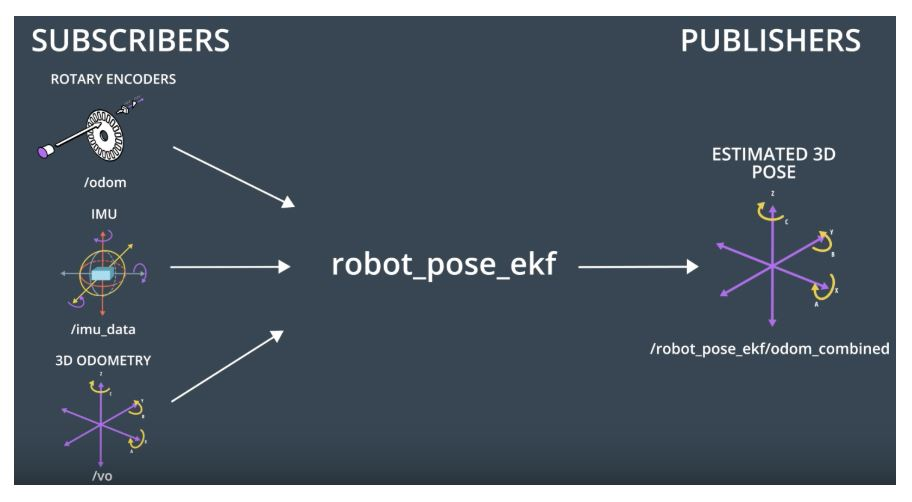
\includegraphics[width=.9\textwidth]{images/Alaa/rosPackage.JPG}%
     % you need to add the caption for the list of figures
    \caption[robot pose ekf packge]{The "robot\_pose\_ekf" package structure.}\label{fig: robot pose ekf packge}%
  \end{figure}
  
  
\subsubsection{Tuning Parameters}
\hspace{2cm} 
first, in order to match the package with our robot, we changed the covariance matrices of the sensors which represent the uncertainty of sensor's readings to some values that suit our sensor's readings.
\par 
\textbf{Hint}: we add such a big value (e.g. 9999) in the covariance matrix in the dimension that is ignored by the sensor. For example if wheel odometry is not giving a reading in Z direction then add to this cell a big number to be ignored.

\par
Second, we replace visual odometry by GPS sensor. A GPS sensor measures the robot 3d position, but not its orientation. The odometry message sent by the GPS sensor could look something like this:

 \begin{figure}[H]%
    \center%
    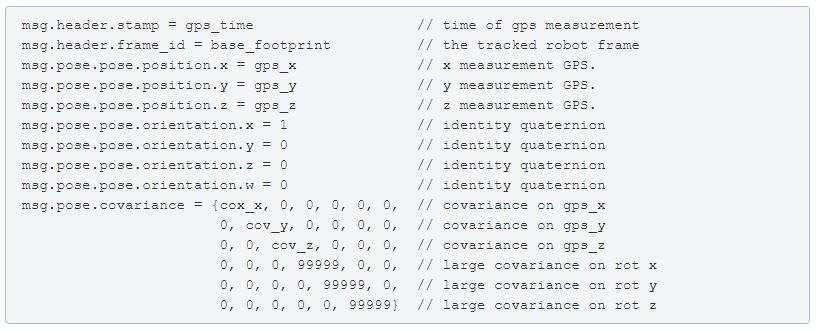
\includegraphics[width=1.0\textwidth]{images/Alaa/gps.JPG}%
     % you need to add the caption for the list of figures
    \caption[GPS message]{GPS message.}\cite{web037}\label{fig: GPS message}%
  \end{figure}

